\documentclass{scrartcl}

\usepackage{graphicx} % Required for the inclusion of images

\renewcommand{\labelenumi}{\alph{enumi}.}
% deutsche Sprache und Umlaute
\usepackage[utf8x]{inputenc}
\usepackage[ngerman]{babel}


%BibTex verweise
\usepackage{cite}

% für url pfade
\usepackage[hyphens]{url}

% setzt beim neuen Absatz das erste Wort 4 mm nach rechts \\ kleine Abstand vom Rand
\setlength{\parindent}{4mm}

%für boxen
\usepackage{pifont,mdframed}

\usepackage{microtype}

% hack für scr paket für Indexierung
\usepackage{scrhack}

% erzwingen der Positionierung
\usepackage{float}
\restylefloat{figure}

% Verbindungen vom Index, Tabellen und Abbildungen
\usepackage{hyperref}

%Tiefe des Inhaltsverzeichnis
\setcounter{tocdepth}{5}

%für Unterstriche
\usepackage{underscore}

% Beschriftung
\usepackage{caption}
\captionsetup{%
  font=small,
  labelfont=bf,
}

\usepackage{fancybox}

%\geometry{showframe}% for debugging purposes -- displays the margins

\usepackage{amsmath}
\usepackage{amssymb}
\usepackage{geometry}
\geometry{verbose,a4paper,tmargin=20mm,bmargin=25mm,lmargin=15mm,rmargin=20mm}
% Set up the images/graphics package

% The following package makes prettier tables.  We're all about the bling!
\usepackage{booktabs}

% The units package provides nice, non-stacked fractions and better spacing
% for units.
\usepackage{units}

% The fancyvrb package lets us customize the formatting of verbatim
% environments.  We use a slightly smaller font.
\usepackage{fancyvrb}
\fvset{fontsize=\normalsize}

% Small sections of multiple columns
\usepackage{multicol}

% Provides paragraphs of dummy text
\usepackage{lipsum}

% listing
\usepackage{listings}
\usepackage{color}
\definecolor{grey}{rgb}{0.4,0.4,0.4}
\definecolor{darkblue}{rgb}{0.0,0.0,0.6}
\definecolor{cyan}{rgb}{0.0,0.6,0.6}

\lstset{
  basicstyle=\tiny,
  columns=fullflexible,
  showstringspaces=false,
  commentstyle=\color{gray}\upshape
}

\lstdefinelanguage{XML} {
  morestring=[b]",
  morestring=[s]{>}{<},
  morecomment=[s]{<?}{?>},
  stringstyle=\color{black},
  identifierstyle=\color{darkblue},
  keywordstyle=\color{cyan},
  morekeywords={xmlns,version,type}
}

\makeatletter
\newenvironment{CenteredBox}{%
\begin{Sbox}}{% Save the content in a box
\end{Sbox}\centerline{\parbox{\wd\@Sbox}{\TheSbox}}}% And output it centered
\makeatother



\title{Rechnersicherheit - Übung 10}
\author{Martin Görick, Dennis Hägler und Kai Kriedemann \\ Tutor: Stefan Pfeiffer}
%\date{\today}  % if the \date{} command is left out, the current date will be used


\begin{document}
\maketitle


\section*{Aufgabe 1 - Bell-LaPadula}


\section*{Aufgabe 2 - Chinese Wall}

\begin{center}
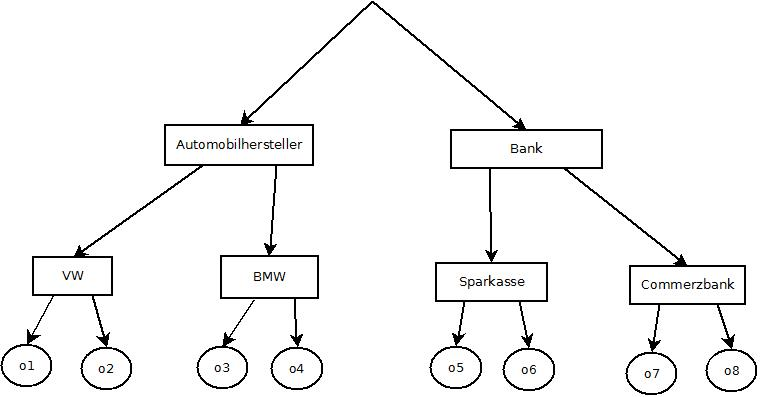
\includegraphics[scale=0.7]{Diagramm1.jpeg}
\end{center}

Oben ein Beispiel mit zwei Konfliktklassen, 4 Firmen (2 pro Klasse) und jeweils 2 sensiblen Objekten pro Firma. Die Branchen sind dabei einmal Banken und einmal Automobilhersteller. Die verschiedenen Branchen entsprechen dabei den Konfliktklassen.

Die beiden Regeln des Chinese-Wall-Modells sagen nun folgendes aus:
\begin{enumerate}
\item Eine Person hat das Recht zur Zeit t, o1 lesen zu dürfen. Voraussetzung dessen: Bisher hat diese Person auf kein o einer anderen Firma innerhalb derselben Konfliktklasse zugegriffen (hier: o3 oder o4). Nach dem Lesen von o1 trifft nun der Namensgeber dieses Modells in Kraft: da die besagte Person nun o1 gelesen hat, darf sie nicht mehr o3 bzw. o4 lesen. Dies würde nämlich dann die ss-property verletzen. Durch den vorherigen Zugriff auf o1 verbauen wir uns den Zugriff auf o3 und o4 und haben uns quasi eine Mauer drum herum gebaut. Noch haben wir keinerlei Einschränkungen für die zweite Konfliktklasse "Bank". Hier könnte man also eine weitere Firma beraten (z.B. Sparkasse). Durch das Leserecht dieser Bank  haben wir jedoch auch kein Recht auf andere Banken (hier: Commerzbank). Andere sensible Daten derselben Firma dürfen natürlich weiterhin gelesen werden. Für unser Beispiel belassen wir die Leserechte unseres Beraters aber bei o1 und o2, also VW.

\item Das Recht, auf ein o zu schreiben, ist nur dann gestattet, wenn man bisher nur Lesezugriff auf sensible Daten ein- und derselben Firma hatte. In unserem Beispiel darf der vorher genannte Berater nur auf o1 oder o2 schreiben. Auf o3 und o4 hat er nicht einmal ein Leserecht (siehe vorher), auf o5 bis o8 darf er auch kein Leserecht besitzen. Die *-property restriktiert dies komplett auf Objekte einer Firma.  Bemerkenswert ist hier also, dass dieser Berater selbst kein Lese- und Schreibrecht auf Objekte einer anderen Branche (bzw. Konfliktklasse) haben darf.  Somit haben wir uns mit dem Schreiben den Zugriff auf andere Firmen (sogar anderer Konfliktklassen) verbaut - lesen und schreiben. Hätte ein Berater Leserecht auf die sensiblen Objekte von VW und z.B. der Sparkasse, so darf er auf keinem der Objekte schreiben. Ausnahme sind natürlich nichtsensible - öffentliche - Daten.

\end{enumerate}

Gehört in diesem Beispiel als Berater lediglich eine lesende Funktion, so bräuchte man mindestens 2 Berater für 4 Firmen. Bei genau 2 Beratern müssen diese natürlich aus jeder Konflitklasse unterschiedliche Firmen beraten (z.B. Berater 1 nimmt VW und die Sparkasse, Berater 2 BMW und die Commerzbank).

Gehört jedoch auch das Schreiben dazu (was als Berater höchstwahrscheinlich der Fall ist) brauchen wir pro Firma 1 Berater, in diesem Beispiel also 4.


\section*{Aufgabe 3 - Informationsfluss 1}

Könnte eigentlich nur passieren, wenn lediglich ein Branch der if-Anweisung ausgeführt wird, und der andere nicht in Betrachtung kommt. Dafür im Code zu sorgen, dass die Abfrage in der Bedingungsüberprüfung immer nur in einem Wert resultiert, macht wenig Sinn, denn dann könnte man es gleich weglassen. Etwas anderes wäre, wenn diese Variable in der Bedigung z.B. in einer externen Datei- einer config-Datei – fix initialisiert ist. Darauf hat der compiler keinen Einfluss und weiß somit natürlich nicht, dass ein Branch der if-Anweisung niemals ausgeführt wird, da die in der Config vorgegebene Bedingungsvariable immer nur einen Wert hat. Ist aber in dem nicht ausgeführten Branch eine Variable y, welche kleiner ist als x (in Bezug auf deren Sicherheitsklassen), so wird dies vom Compiler nicht erlaubt werden. Durch die Nichttraversierung des Branches findet jedoch kein unerlaubter Informationsfluss statt.

\section*{Aufgabe 4 - Informationsfluss 2}

H(x) = - $\sum_{x \in \mathfrak{X}  } Pr(X = x) \cdot log_{2} Pr(X=x)$

Pr(X=x) beträgt $\frac{1}{2}^n$ für alle  $x \in \{0,1\}^n$. Der Term des Informationsgehaltes -  $ log_{2} Pr(X=x)$ - beträgt dabei in diesem Fall immer -n.  $ log_{2} Pr(X=x)$ lässt sich auch schreiben als  $ log_{2} \frac{1}{2}^n = \frac{log \frac{1}{2}^n}{log_2} =  \frac{log 2^{-n}}{log_2} = -n.$

H(x) in diesem Beispiel lautet also - $\sum_{x \in \mathfrak{X} } \frac{1}{2}^n \cdot (-n)$. Die Anzahl der Summanden beträgt $2^n$, also: $- 2^n \cdot \frac{1}{2}^n \cdot (-n)$ und dies lässt sich zusammenfassen als $(-1)^n * (-n) = n$. Somit beträgt die Entropie in diesem Beispiel immer die Länge unseres Bitstrings. In der VL hatten wir das Beispiel Münzwurf, dort hat unser n und dessen Entropie den Wert 1 betragen. 






\end{document}